\documentclass[11pt,a4paper]{article}
\usepackage[margin=2.3cm]{geometry}
\usepackage[T1]{fontenc}
\usepackage{amsmath,amssymb}
\usepackage{graphicx}
\usepackage{booktabs}
\usepackage{float}
\usepackage{caption}
\usepackage{enumitem}
\usepackage{tikz}
\usetikzlibrary{positioning,arrows.meta}
\usepackage[hidelinks]{hyperref}
\usepackage{setspace}
\setstretch{1.08}
\setlength{\parskip}{3pt}
\captionsetup{font=small,labelfont=bf}
\setlist{itemsep=1pt,topsep=2pt}

% Draw a figure if the image file exists, otherwise a clearly marked placeholder box
\newcommand{\safefig}[3]{%
  \IfFileExists{#1}{\includegraphics[width=#2\linewidth]{#1}}{%
  \fbox{\parbox{#2\linewidth}{\centering\vspace{1.2cm}\texttt{\detokenize{#1}}\\(upload this image to the project)\vspace{1.2cm}}}}}

\begin{document}

%--------------------------------------------------------------- TITLE
\begin{center}
{\large\textbf{Manipal University Jaipur}}\\[2pt]
Department of Data Science and Engineering\\[10pt]
\rule{\linewidth}{0.6pt}\\[6pt]
{\LARGE\bfseries Deepfake Video Detection Using\\[2pt] Spatio-Temporal Features and a\\[2pt] Dynamic Difference Module}\\[4pt]
{\large A re-implementation and critical evaluation}\\[2pt]
\rule{\linewidth}{0.6pt}\\[8pt]
\textbf{Computer Vision Course Project}\\[8pt]
\begin{tabular}{ccc}
\textbf{Harshita Chokhani} & \hspace{2em} & \textbf{Vanshika Saini}\\
2430010505 & & 2430010523\\
\end{tabular}\\[8pt]
Under the guidance of \textbf{Dr.\ Ashish Pandey}\\[2pt]
October 2026
\end{center}

\begin{abstract}
\noindent Deepfake videos are produced frame by frame, so they often contain small geometric and temporal inconsistencies that a viewer does not notice. AbdElfattah et al.\ (Scientific Reports, 2026) propose a detector that combines VGG16 frame features, Dlib facial-landmark geometry, an LSTM, a Transformer encoder and a Dynamic Difference Module (DDM) that measures abrupt frame-to-frame change, and they report accuracies close to 100\% on three benchmarks. In this project we re-implemented that pipeline from the paper's description using PyTorch and trained it on the DFDC face-crop training sample from Kaggle. We describe every stage, state which settings come from the paper and which we had to assume, and report the results of the full model and of the paper's ablation. On our balanced subset (116 videos, 24 of them held out for testing) the model did not generalise: test accuracy was 50\%, and the model gave almost the same score to every video. We discuss why this probably happened, which details the paper leaves open, and what would be needed for a fair reproduction.
\end{abstract}

%--------------------------------------------------------------- 1
\section{Introduction}
Face-swapping and face-reenactment methods can now produce videos that are hard to tell apart from real recordings, which makes automatic detection an important problem for media forensics. Early detectors worked on single frames, but a video is a sequence, and generators usually process each frame almost independently. The result is that small details such as the position of the mouth corners, the spacing of the eyes, or the smoothness of motion can change slightly from one frame to the next in a way that natural video does not.

The paper we studied~\cite{abdelfattah2026} builds a detector around this idea. It extracts appearance features with a CNN, extracts geometric features from 68 facial landmarks, models time with an LSTM and a Transformer encoder, and adds a Dynamic Difference Module that summarises how much the features change between consecutive frames. Our goals were to (i) implement this pipeline end to end, (ii) run it on a publicly available dataset on ordinary hardware, (iii) repeat the paper's ablation study, and (iv) record honestly how close we could get to the published behaviour.

%--------------------------------------------------------------- 2
\section{Dataset}
We used the \emph{DFDC faces of the train sample} dataset on Kaggle, which contains faces already extracted from the training sample of the Deepfake Detection Challenge~\cite{dfdc}. The frames are stored in two folders, \texttt{real} and \texttt{fake}. After grouping frames by video we found 286 videos (228 fake, 58 real), with 180 to 636 frames per video (mean 328).

The dataset is heavily skewed towards fake videos. Following the paper, we balanced the classes by randomly keeping as many fake videos as there are real ones, which gives 58 + 58 = 116 videos. We then split by \emph{video}, never by frame, so that frames of the same clip cannot appear in both training and test data: 80\% for training and 20\% for testing (24 test videos, 12 per class), and a further 10\% of the training part (10 videos) for validation and early stopping. The split is stratified and uses a fixed random seed.

%--------------------------------------------------------------- 3
\section{Methodology}
Figure~\ref{fig:pipeline} shows the pipeline. Each video is turned into a sequence of $T=60$ enhanced face images and 28 geometric features per frame; the images go through a frozen VGG16, and the combined features are modelled over time before the DDM and the final classifier.

\begin{figure}[H]
\centering
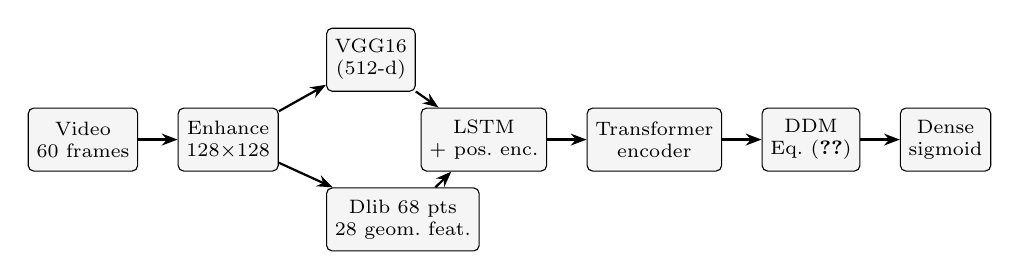
\begin{tikzpicture}[node distance=5mm, every node/.style={font=\scriptsize},
  blk/.style={draw, rounded corners=2pt, minimum height=8mm, align=center, inner sep=3pt, fill=gray!8},
  arr/.style={-{Stealth[length=2mm]}, thick}]
\node[blk] (a) {Video\\60 frames};
\node[blk, right=of a] (b) {Enhance\\128$\times$128};
\node[blk, above right=2mm and 6mm of b] (c) {VGG16\\(512-d)};
\node[blk, below right=2mm and 6mm of b] (d) {Dlib 68 pts\\28 geom.\ feat.};
\node[blk, right=18mm of b] (e) {LSTM\\+ pos.\ enc.};
\node[blk, right=of e] (f) {Transformer\\encoder};
\node[blk, right=of f] (g) {DDM\\Eq.~(\ref{eq:ddm})};
\node[blk, right=of g] (h) {Dense\\sigmoid};
\draw[arr] (a)--(b); \draw[arr] (b)--(c); \draw[arr] (b)--(d);
\draw[arr] (c)--(e); \draw[arr] (d)--(e);
\draw[arr] (e)--(f); \draw[arr] (f)--(g); \draw[arr] (g)--(h);
\end{tikzpicture}
\caption{Overview of the implemented detector.}
\label{fig:pipeline}
\end{figure}

\subsection{Frame sampling and enhancement}
From each video we take $T=60$ frames at evenly spaced positions, $\text{idx}_k=\operatorname{round}\big(k\,(N-1)/(T-1)\big)$, $k=0,\dots,T-1$. Each face image is enhanced as in the paper: it is converted from RGB to YCrCb,
\begin{equation}
[Y,\,C_r,\,C_b]^{\top}=f_{\text{color}}(R,G,B),
\end{equation}
contrast-limited adaptive histogram equalisation (CLAHE)~\cite{clahe} is applied to the brightness channel $Y$ only (tile histogram $h(i)=\sum_{(x,y)\in \text{tile}}\delta\big(I(x,y)-i\big)$), and the image is converted back to RGB. A Non-Local Means filter~\cite{nlm} removes noise while keeping edges, and finally saturation and value are raised in HSV space. The result is resized to $128\times128$. Examples are shown in Figure~\ref{fig:prep}.

\begin{figure}[H]
\centering
\safefig{figure_01.png}{0.8}{}
\caption{Top row: original face crops. Bottom row: the same frames after enhancement and resizing.}
\label{fig:prep}
\end{figure}

\subsection{Landmark geometry}
The Dlib shape predictor~\cite{dlib} returns 68 landmarks $P_i=(x_i,y_i)$, $i=0,\dots,67$ (Figure~\ref{fig:lm}). Raw coordinates change with head position and image size, so, as the paper argues, we compute distances and angles instead. The Euclidean distance between two landmarks is
\begin{equation}
d(P_1,P_2)=\sqrt{(x_2-x_1)^2+(y_2-y_1)^2},
\end{equation}
and the angle at a vertex $B$ between points $A$ and $C$ is
\begin{equation}
\theta=\arccos\!\left(\frac{\vec{BA}\cdot\vec{BC}}{\lVert\vec{BA}\rVert\,\lVert\vec{BC}\rVert}\right).
\end{equation}
We use 20 distances (eye--eye, eye widths and heights, nose--mouth, mouth width and height, nose--chin, cheek--cheek, jaw width and others) and 8 angles (for example right eye--nose tip--left eye and the mouth-corner angles), giving a 28-dimensional vector per frame. Distances are divided by the face width so that they do not depend on scale. The paper names the kinds of measurement but not the full list, so the exact list is our choice. The features are standardised with statistics computed on the training videos only.

\begin{figure}[H]
\centering
\safefig{figure_02.png}{0.22}{}
\caption{The 68 Dlib landmarks drawn on an enhanced face.}
\label{fig:lm}
\end{figure}

\subsection{Spatial features and LSTM}
The convolutional layers of VGG16, pretrained on ImageNet with the fully connected layers removed, produce a feature map for each frame. Global average pooling turns it into a vector $f_t\in\mathbb{R}^{512}$, so a video is described by $F=\{f_1,\dots,f_T\}$. We concatenate the 28 geometric features, giving a 540-dimensional input per frame. (How the two feature types are joined is not stated in the paper; per-frame concatenation is our reading.) The sequence is processed by an LSTM that returns its hidden state at every step,
\begin{equation}
h_t=\text{LSTM}(f_t,h_{t-1}),\qquad H=\{h_1,\dots,h_T\},\ h_t\in\mathbb{R}^{128}.
\end{equation}

\subsection{Transformer encoder}
Sinusoidal positional encoding is added to keep frame order, $X=H+PE$, with $PE(pos,2i)=\sin\!\big(pos/10000^{2i/d}\big)$ and $PE(pos,2i{+}1)=\cos\!\big(pos/10000^{2i/d}\big)$. The encoder block uses multi-head self-attention,
\begin{equation}
\text{Attention}(Q,K,V)=\operatorname{softmax}\!\left(\frac{QK^{\top}}{\sqrt{d_k}}\right)V,\qquad Q=XW_Q,\ K=XW_K,\ V=XW_V,
\end{equation}
followed by a feed-forward network
\begin{equation}
\text{FFN}(p)=W_2\,\operatorname{ReLU}(W_1p+b_1)+b_2 ,
\end{equation}
with dropout, a residual connection and layer normalisation after each part. We use 4 heads, one block and a feed-forward width of 128.

\subsection{Dynamic Difference Module}
Let $S\in\mathbb{R}^{T\times D}$ be the Transformer output. The DDM computes the average absolute change of every feature between consecutive frames,
\begin{equation}
Z=\frac{1}{T-1}\sum_{t=1}^{T-1}\left|S_{t+1}-S_t\right| ,\label{eq:ddm}
\end{equation}
so that sudden, unnatural changes receive a large value while smooth natural motion gives a small one. The vector $Z\in\mathbb{R}^{128}$ is passed to the classifier. (The paper also describes concatenating $z_t$ with $d_t=|z_t-z_{t-1}|$; we implemented both readings, and used the averaged form of Eq.~(\ref{eq:ddm}) because it is the one written as the module's definition.)

\subsection{Classifier, loss and training}
A dense layer with 64 units and ReLU, dropout 0.5 and a final sigmoid unit give $\hat y=\sigma(w^{\top}a+b)$, the probability that the video is fake. Training minimises binary cross-entropy,
\begin{equation}
\mathcal{L}=-\big[\,y\log\hat y+(1-y)\log(1-\hat y)\,\big],
\end{equation}
and a video is labelled fake when $\hat y>0.5$, as in the paper. The metrics are accuracy $=(TP+TN)/(TP+TN+FP+FN)$, precision $=TP/(TP+FP)$, recall $=TP/(TP+FN)$ and $F_1=2PR/(P+R)$.

%--------------------------------------------------------------- 4
\section{Implementation details}
The system is written in Python with PyTorch 2.15, torchvision, OpenCV, Dlib and scikit-learn, and was trained on a laptop GPU through Apple's MPS backend. Preprocessed frames and features are cached so that the expensive enhancement step runs once. A separate script classifies new \texttt{.mp4} files: it finds the face with MTCNN~\cite{mtcnn}, applies the same preprocessing and returns $P(\text{fake})$. Table~\ref{tab:cfg} lists the settings and where each comes from.

\begin{table}[H]
\centering\small
\caption{Training configuration and the origin of each setting.}
\label{tab:cfg}
\begin{tabular}{@{}p{4.9cm}p{5.6cm}p{4.9cm}@{}}
\toprule
Setting & Value & Source\\
\midrule
Frames per video & 60 & paper\\
Input size & $128\times128$ & paper\\
Backbone & VGG16, no FC layers & paper (frozen: our choice)\\
Optimiser, learning rate & Adam~\cite{adam}, $10^{-3}$ & rate: paper; Adam: our choice\\
Batch size, epochs & 32, up to 12 & paper (best DFDC setting)\\
Dropout & 0.5 & paper\\
Augmentation & flip, rotation $\pm10^\circ$, brightness $\times0.8$--$1.2$ & paper (ranges ours)\\
Early stopping & validation loss, patience 5 & paper (patience ours)\\
Split & 80:20, balanced classes & paper\\
LSTM units; heads; blocks; FFN width & 128; 4; 1; 128 & our choice\\
CLAHE clip / tiles; NLM strength & 2.0 / $8\times8$; 5 & our choice\\
Landmark feature list & 20 distances + 8 angles & kinds: paper; list: ours\\
\bottomrule
\end{tabular}
\end{table}

%--------------------------------------------------------------- 5
\section{Results}
Table~\ref{tab:abl} gives the test results of the full model and the three ablation variants of the paper (without the Transformer encoder, without the DDM, and without landmark features). Every variant was trained with the same seed and data split.

\begin{table}[H]
\centering\small
\caption{Test-set results (24 videos, 12 real and 12 fake).}
\label{tab:abl}
\begin{tabular}{@{}lcccc@{}}
\toprule
Model & Accuracy & Precision & Recall & F1\\
\midrule
Full (LSTM + Transformer + DDM + landmarks) & 0.5000 & 0.5000 & 1.0000 & 0.6667\\
Without Transformer encoder & 0.4583 & 0.4667 & 0.5833 & 0.5185\\
Without DDM & 0.4583 & 0.4667 & 0.5833 & 0.5185\\
Without landmark features & 0.5000 & 0.5000 & 1.0000 & 0.6667\\
\bottomrule
\end{tabular}
\end{table}

For the full model, precision 0.5 and recall 1.0 on a balanced test set mean that all 24 videos were labelled fake. Figure~\ref{fig:res} shows the training curves and the confusion matrix.

\begin{figure}[H]
\centering
\safefig{full_curves.png}{0.62}{}\hfill
\safefig{confusion.png}{0.33}{}
\caption{Left: training and validation accuracy and loss of the full model. Right: confusion matrix on the test videos.}
\label{fig:res}
\end{figure}

\textbf{Reading the numbers.} The test set has only 24 videos, so one video changes accuracy by $4.2$ percentage points; the difference between 0.500 and 0.458 is a single video and does not show that any component helps or hurts. More telling is the behaviour during training: training accuracy rose clearly above chance (the no-landmark variant, for example, ended at 75.6\%), while validation accuracy stayed at 50\% and validation loss stayed close to $\ln 2\approx0.693$. At inference the full model returned about $0.52$--$0.53$ for both real and fake clips, which the 0.5 threshold turns into ``fake'' for almost everything. In short, the network memorised the 82 training videos and learned nothing that carried over to unseen ones.

%--------------------------------------------------------------- 6
\section{Discussion}
\subsection{Why our results differ from the paper}
The paper reports up to 100\% accuracy on DFDC and FaceForensics++ and 99.6\% on UADFV. We did not reproduce this, and we think several factors contribute.
\begin{itemize}
\item \textbf{Very little data.} Only 58 real videos exist in the sample, so training used 82 videos. A model with a recurrent layer and a Transformer on top of 540-dimensional inputs overfits quickly at this size.
\item \textbf{Weak features.} With a frozen ImageNet VGG16 and global average pooling at $128\times128$, the subtle blending and texture artefacts of deepfakes are largely averaged away, and our landmark features carry little signal on their own.
\item \textbf{Different data and protocol.} The paper's DFDC experiments use small hand-picked subsets of 60 to 400 videos, and the text does not explain how frames or clips were separated between training and validation. If frames of the same video appear on both sides, training and validation scores become artificially high; we cannot verify whether this happened, but it would explain the gap between 98--100\% and our 50\%.
\end{itemize}

\subsection{Details missing from the paper}
The method description leaves several choices open: the LSTM size, number of attention heads and layers, the exact landmark measurements, how landmark features are fused with CNN features, the CLAHE and denoising strengths, the optimiser, and whether the backbone is fine-tuned. No code is released. Table~\ref{tab:cfg} marks every such choice, and a different choice could change the outcome. The paper also states that the model is saved after training and ``classification report is printed'', but gives no confusion matrix for the main benchmarks and no cross-dataset test with a separate split.

\subsection{Limitations of this work}
Our experiment used only the DFDC sample (not FaceForensics++ or UADFV), a balanced set of 116 videos, a 24-video test set, a single random seed, and a laptop GPU. The test results therefore carry a large uncertainty and should not be read as an estimate of the method's true performance.

\subsection{Possible improvements}
(i) Use all 286 videos with class-weighted loss and report AUC as well as accuracy; (ii) fine-tune the CNN instead of freezing it, or use a stronger backbone; (iii) cut each video into several clips so that more training sequences exist while still splitting by video; (iv) repeat with several seeds and report mean and spread; (v) test on a second dataset to measure generalisation.

%--------------------------------------------------------------- 7
\section{Conclusion}
We implemented the complete detector described by AbdElfattah et al., from frame enhancement and landmark geometry through VGG16, LSTM, Transformer encoder and Dynamic Difference Module to classification, together with the paper's ablation and a script for classifying new videos. The code runs end to end on a standard laptop. On the DFDC sample the trained model performed at chance level, so we could not confirm the published accuracy. We believe the main causes are the small number of real videos, the frozen general-purpose features, and under-specified details and evaluation protocol in the original paper. The project still gave us a working, documented pipeline, a clear list of the paper's open points, and a concrete plan for a fairer reproduction.

%--------------------------------------------------------------- refs
\begin{thebibliography}{99}\small
\bibitem{abdelfattah2026} E.~AbdElfattah, H.~M.~Mousa, A.~Elsisi, N.~Mahmoud. Robust deepfake video detection using spatio-temporal features and dynamic difference learning. \emph{Scientific Reports}, 2026. doi:10.1038/s41598-026-53545-w.
\bibitem{dfdc} B.~Dolhansky et al. The DeepFake Detection Challenge (DFDC) dataset. arXiv:2006.07397, 2020.
\bibitem{vgg} K.~Simonyan, A.~Zisserman. Very deep convolutional networks for large-scale image recognition. \emph{ICLR}, 2015.
\bibitem{lstm} S.~Hochreiter, J.~Schmidhuber. Long short-term memory. \emph{Neural Computation}, 9(8):1735--1780, 1997.
\bibitem{transformer} A.~Vaswani et al. Attention is all you need. \emph{NeurIPS}, 2017.
\bibitem{dlib} D.~E.~King. Dlib-ml: a machine learning toolkit. \emph{JMLR}, 10:1755--1758, 2009.
\bibitem{mtcnn} K.~Zhang, Z.~Zhang, Z.~Li, Y.~Qiao. Joint face detection and alignment using multitask cascaded convolutional networks. \emph{IEEE Signal Processing Letters}, 23(10):1499--1503, 2016.
\bibitem{clahe} K.~Zuiderveld. Contrast limited adaptive histogram equalization. In \emph{Graphics Gems IV}, pp.\ 474--485, Academic Press, 1994.
\bibitem{nlm} A.~Buades, B.~Coll, J.-M.~Morel. A non-local algorithm for image denoising. \emph{CVPR}, 2005.
\bibitem{adam} D.~P.~Kingma, J.~Ba. Adam: a method for stochastic optimization. \emph{ICLR}, 2015.
\end{thebibliography}

\end{document}
